<<<<<<< local
% Her skal billeder/figurer inds�ttes med et referencenummer under. (fx. Figur 9.3)

\begin{center}

	\textbf{F�rste prototype}
    \label{1Prototype}
	
	
   	\includegraphics{1.Prototype/Login_Vindue}\\
   		{\small \textit{Figur 1: login Vindue 1.Prototype}}

\leavevmode \linebreak   		
   		
   	\includegraphics{1.Prototype/Login_Vindue_Info}\\
   	   	{\small \textit{Figur 2: login Vindue med info 1.Prototype}}
   	   	
\leavevmode \linebreak

	\includegraphics[height= 185px]{1.Prototype/Status_Vindue}\\
		{\small \textit{Figur 3: Status Vindue 1.Prototype}}

	\textbf{Anden prototype}
	
	
	\includegraphics{2.Prototype/Login_Vindue}\\
		{\small \textit{Figur 4: Login Vindue 2.Prototype}}

\leavevmode \linebreak

	\includegraphics{2.Prototype/Login_Vindue_Info}\\
		{\small \textit{Figur 5: Login Vindue med info 2.Prototype}}

\leavevmode \linebreak

	\includegraphics[height= 200px]{2.Prototype/Status_Vindue}\\
		{\small \textit{Figur 6: Status Vindue 2.Prototype}}


	
\includegraphics{2.Prototype/TrayIcon}\\
		{\small \textit{Figur 7: Tray Icon 2.Prototype}}

\leavevmode \linebreak

	\includegraphics{2.Prototype/TrayIconMenu}\\
		{\small \textit{Figur 8: Tray Icon menu 2.Prototype}}


\leavevmode \linebreak

	\textbf{Tredje prototype}
	
	
   	\includegraphics{3.Prototype/Login_Vindue}\\
   		{\small \textit{Figur 9: Login Vindue 3.Prototype}}

\leavevmode \linebreak

	\includegraphics[height= 110px]{3.Prototype/Login_Vindue_Info}\\
		{\small \textit{Figur 10: Login Vindue Info 3.Prototype}}


	\includegraphics{3.Prototype/Status_Vindue}\\
		{\small \textit{Figur 11: Status Vindue 3.Prototype}}

\leavevmode \linebreak

	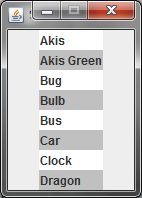
\includegraphics{3.Prototype/Add_Vindue}\\
		{\small \textit{Figur 12: Add Vindue 3.Prototype}}

\leavevmode \linebreak

	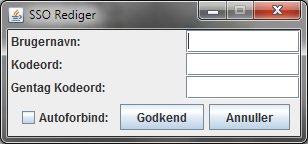
\includegraphics{3.Prototype/Edit_Vindue}\\
		{\small \textit{Figur 13: Edit Vindue 3.Prototype}}

	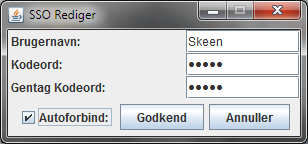
\includegraphics{3.Prototype/Edit_Vindue_Info}\\
		{\small \textit{Figur 14: Edit Vindue Info 3.Prototype}}

\leavevmode \linebreak

	
\includegraphics{3.Prototype/TrayIcon}\\
		{\small \textit{Figur 15: Tray Icon 3.Prototype(2. ikon fra venstre)}}

\leavevmode \linebreak

	\includegraphics{3.Prototype/TrayIconMenu}\\
		{\small \textit{Figur 16: Tray Icon menu 3.Prototype}}

\end{center}

=======
% Her skal billeder/figurer inds�ttes med et referencenummer under. (fx. Figur 9.3)

\begin{center}

	\textbf{F�rste prototype}
    \label{1Prototype}
	
	
   	\includegraphics{1.Prototype/Login_Vindue}\\
   		{\small \textit{Figur 1: login Vindue 1.Prototype}}

\leavevmode \linebreak   		
   		
   	\includegraphics{1.Prototype/Login_Vindue_Info}\\
   	   	{\small \textit{Figur 2: login Vindue med info 1.Prototype}}
   	   	
\leavevmode \linebreak

	\includegraphics[height= 185px]{1.Prototype/Status_Vindue}\\
		{\small \textit{Figur 3: Status Vindue 1.Prototype}}

	\textbf{Anden prototype}
	
	
	\includegraphics{2.Prototype/Login_Vindue}\\
		{\small \textit{Figur 4: Login Vindue 2.Prototype}}

\leavevmode \linebreak

	\includegraphics{2.Prototype/Login_Vindue_Info}\\
		{\small \textit{Figur 5: Login Vindue med info 2.Prototype}}

\leavevmode \linebreak

	\includegraphics[height= 200px]{2.Prototype/Status_Vindue}\\
		{\small \textit{Figur 6: Status Vindue 2.Prototype}}


	
\includegraphics{2.Prototype/TrayIcon}\\
		{\small \textit{Figur 7: Tray Icon 2.Prototype}}

\leavevmode \linebreak

	\includegraphics{2.Prototype/TrayIconMenu}\\
		{\small \textit{Figur 8: Tray Icon menu 2.Prototype}}


\leavevmode \linebreak

	\textbf{Tredje prototype}
	
	
   	\includegraphics{3.Prototype/Login_Vindue}\\
   		{\small \textit{Figur 9: Login Vindue 3.Prototype}}

\leavevmode \linebreak

	\includegraphics[height= 110px]{2.Prototype/Login_Vindue_Info}\\
		{\small \textit{Figur 10: Login Vindue Info 3.Prototype}}


	\includegraphics{3.Prototype/Status_Vindue}\\
		{\small \textit{Figur 11: Status Vindue 3.Prototype}}

\leavevmode \linebreak

	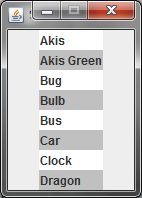
\includegraphics{3.Prototype/Add_Vindue}\\
		{\small \textit{Figur 12: Add Vindue 3.Prototype}}

\leavevmode \linebreak

	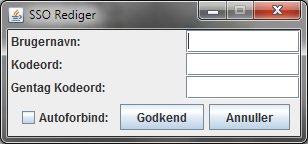
\includegraphics{3.Prototype/Edit_Vindue}\\
		{\small \textit{Figur 13: Edit Vindue 3.Prototype}}

	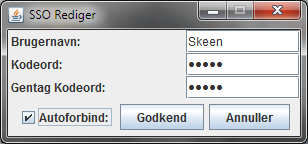
\includegraphics{3.Prototype/Edit_Vindue_Info}\\
		{\small \textit{Figur 14: Edit Vindue Info 3.Prototype}}

\leavevmode \linebreak

	
\includegraphics{3.Prototype/TrayIcon}\\
		{\small \textit{Figur 15: Tray Icon 3.Prototype}}

\leavevmode \linebreak

	\includegraphics{3.Prototype/TrayIconMenu}\\
		{\small \textit{Figur 16: Tray Icon menu 3.Prototype}}

\end{center}

>>>>>>> other
